\newcommand{\checkbox}[1]{\item[$\square$]\textbf{#1}\\}

\chapter*{Erstsemester-Checkliste}
\addcontentsline{toc}{chapter}{Erstsemester-Checkliste \hspace*{.1cm} \keys{must read}}

Für einen erfolgreichen Start in das Studium solltest du einige organisatorische
Kleinigkeiten unbedingt in den ersten Wochen erledigen. Diese haben wir dir in
folgender Checkliste mit absteigender Priorität zusammengestellt.

\begin{itemize}[leftmargin=*]

\checkbox{Wohnung}
Solltest du noch keine Bleibe gefunden haben, ist Beeilung angesagt, denn die
schönsten Wohnungen sind schnell weg. Wenn du in den Genuss eines
superschnellen Internetzugangs kommen möchtest, seien dir die Wohnheime~\link{https://www.studentenwerk-dresden.de/wohnen/wohnheimkatalog} des
Studierendenwerks empfohlen. Alternativ bieten sich auch Portale wie
\textit{\mbox{WG-Gesucht}}~\link{https://www.wg-gesucht.de/} an.

\checkbox{ZIH-Login aktivieren}
Alle Studierenden erhalten vom \textit{Zentrum für Informationsdienste und
Hochleistungsrechnen}, kurz ZIH, einen Uni-Account. Dieser wird für alle
wichtigen Funktionen rund um das Studium gebraucht, sei es das WLAN auf dem
Campus oder die Anmeldung zu Prüfungen und Lehrveranstaltungen. \\
Damit du diese Dienste nutzen kannst, ist es notwendig deinen ZIH-Login mit dem
IDM-Coupon im \textit{Identity Manager}~\link{https://idm-coupon.tu-dresden.de}
zu aktivieren. Der Coupon sollte an deine im Bewerberportal angegebene
Emailadresse zugestellt worden sein.

\checkbox{E-Mail}
Du bekommst vom ZIH ein Exchange-Postfach \textit{vona123a@msx.tu-dresden.de}
und einen Alias der Form \textit{vorname.nachname@mailbox.tu-dresden.de}.
Ältere Jahrgänge haben E-Mail-Adressen der Form
\textit{s1234567\allowbreak{}@mail.zih.tu-dresden.de}, wundere dich also nicht,
wenn du die noch siehst. Falls dein Name an der TU Dresden bereits existiert,
lautet die Alias-Adresse für Max Mustermann dann z.B.
\textit{max.mustermann1@mailbox…}. \\
Zugriff auf dein Postfach erlangst du per Webmail und IMAP\@. Alternativ kann eine
Weiterleitung an eine persönliche Adresse eingerichtet werden. Vor allem
wichtige E-Mails von der Uni werden an diese Adressen geschickt. Sorge deshalb
dafür, dass du deine Mails regelmäßig abrufst oder an eine andere Adresse
weiterleitest. Weitere Informationen hierzu finden sich unter~\link{https://tu-dresden.de/zih/dienste/service-katalog/arbeitsumgebung/e_mail/}.

\checkbox{BAföG-Antrag}
Die Antragsformulare findest du auf den Seiten des BMBF~\link{https://www.bafög.de/de/alle-antragsformulare-432.php}. Für weitere
Auskünfte steht dir das Servicebüro oder dein Sachbearbeiter im
Studierendenwerk zur Verfügung. Schiebe den Antrag nicht allzu lang vor dir
her, da dein Anspruch frühestens ab dem Antragsmonat gilt. Informationen zu den
Sprechzeiten beim Studierendenwerk gibt es hier~\link{https://www.studentenwerk-dresden.de/finanzierung/servicebuero.html}.

\pagebreak

\checkbox{Wohnsitz anmelden}
Offiziell musst du innerhalb von zwei Wochen beim zuständigen Ortsamt~\link{https://www.dresden.de/de/rathaus/dienstleistungen/wohnsitz_meldung_d115.php}
deine Wohnung anmelden. Wer seinen Hauptwohnsitz nach Dresden verlegt, kann bei
der Stadt eine \enquote{Umzugsbeihilfe} in Höhe von 150\euro\ beantragen.
Informationen dazu gibt's unter~\link{https://www.dresden.de/de/rathaus/dienstleistungen/c_336.php} und~\link{https://www.studentenwerk-dresden.de/wohnen/umzugsbeihilfe.html}. \\
Wenn du deine Wohnung hingegen als Nebenwohnsitz anmeldest, musst du
Zweitwohnungssteuer zahlen. Diese beträgt 10\% der Kaltmiete pro Monat.
Weiteres hierzu findest du auf den Seiten des StuRa~\link{https://www.stura.tu-dresden.de/zweitwohnungssteuer} oder der Stadt
Dresden~\link{https://www.dresden.de/de/rathaus/dienstleistungen/c_zweitwohnungssteuer.php}.

\checkbox{WLAN}
Sowohl auf dem Campus als auch in den Räumlichkeiten der Fakultät kannst du mit
deinen Geräten ins Internet. Das Netzwerk heißt \textit{eduroam} und bietet dir
einen sicheren Internetzugang nicht nur an der TU Dresden, sondern auch an sehr
vielen anderen Universitäten weltweit. Zugang erhältst du mit deinem ZIH-Login,
hier ausnahmsweise in der Form \textit{vona123a@tu-dresden.de}, und deinem
Passwort. Mehr Informationen findest du unter~\link{https://tu-dresden.de/zih/dienste/arbeitsumgebung/zugang_datennetz}.

\checkbox{Emeal-Karte}
Die Mensakarte ermöglicht dir das bargeldlose Bezahlen in den verschiedenen
Mensen der Uni. Du erhältst sie während der ESE oder in den Mensen selbst gegen
eine Kaution von 5\euro\ und unter Vorlage der Emeal-Bescheinigung, die du auf
deinem Semesterbogen findest.

\begin{figure}[b!]
\centering
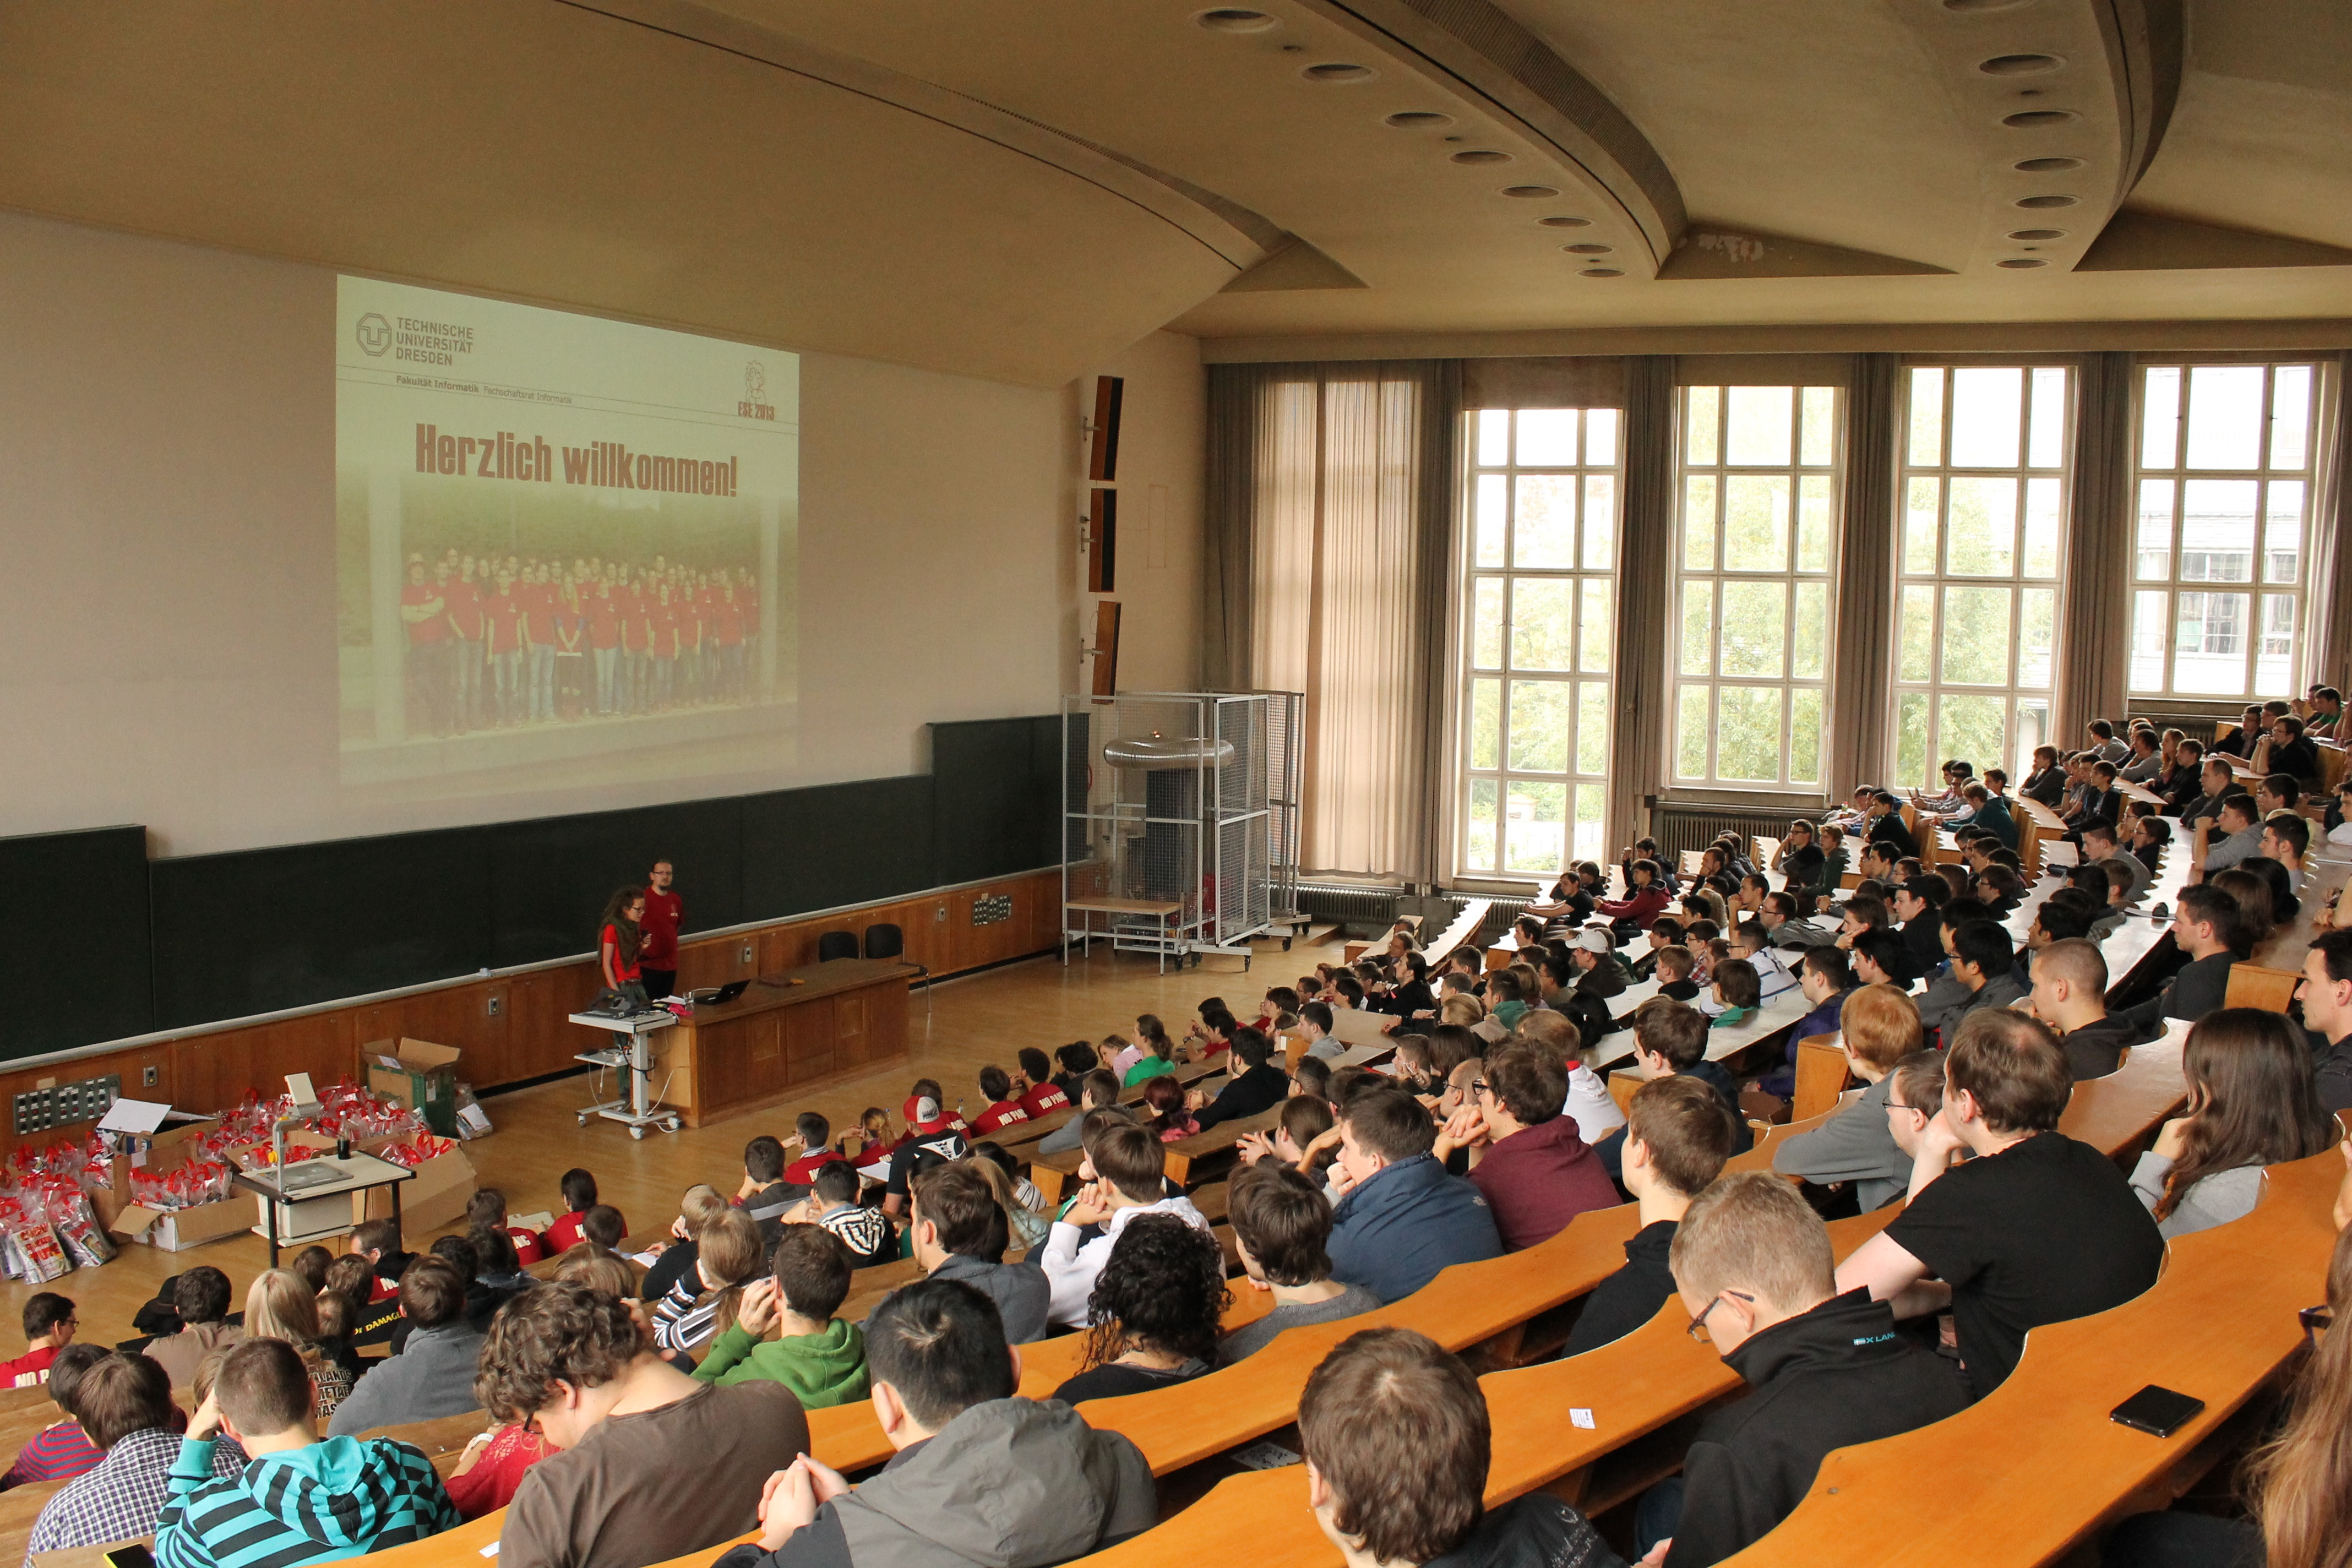
\includegraphics[width=.99\linewidth]{img/ese2013/barschoe.jpg}
\end{figure}

\checkbox{Programmierkurse}
Besonders denjenigen ohne Programmiererfahrung werden die im Wintersemester
angebotenen Programmierkurse ans Herz gelegt. Vor allem der C- und der Java-Kurs
sind sehr hilfreich, um durch die ersten Semester zu kommen. Die Kurse finden in
der Regel unter der Woche statt, manche jedoch auch am Wochenende. Für Details
wende dich an~\link{mailto:programmierung@ifsr.de} oder behalte die News auf der
Seite des FSR~\link{https://www.ifsr.de} im Auge.

\checkbox{(optional) Sprachkurse}
Die TU Dresden bietet Sprachkurse für Englisch und viele weitere Sprachen an.
Die Einschreibung für die Sprachkurse wird je nach Kurs im Laufe der ersten
beiden Wochen deines Studiums freigeschaltet. Erkundige dich auf den Seiten des
LSK~\link{https://tu-dresden.de/gsw/slk/lsk/sprachen-fuer-alle-studiengaenge/einschreibung-ueber-lskonline/} frühzeitig, wann dies ist. Die
meisten Kurse sind sehr schnell voll.

\checkbox{(optional) Sportkurse}
Wie für die Sprachkurse gilt auch hier, wer zuerst da ist\ldots{} Das Angebot
kannst du beim Universitätssportzentrum (USZ) einsehen~\link{https://tu-dresden.de/usz}. Hast du dich für einen Kurs entschieden und
bei freigeschalteter Einschreibung für diesen angemeldet, musst du nur noch die
Anmeldebescheinigung drucken und den Kostenbeitrag innerhalb von drei Tagen auf
das Konto des USZ überweisen.

\checkbox{Studienrelevante Dokumente}
Das Vorlesungsverzeichnis~\link{https://tu-dresden.de/ing/informatik/studium/lehre} und die Prüfungs- und
Studienordnung~\link{https://tu-dresden.de/ing/informatik/studium/studienangebot} erhältst du
auf den Seiten der Fakultät. Gedruckte Ordnungen gibt's beim FSR, werden aber auch während der Seminargruppentreffen verteilt.
Alle wichtigen Informationen zu den einzelnen Vorlesungen findest du
auf den jeweiligen Seiten der Institute im Netz.  Die Professoren werden dir
dazu jedoch auch noch alles in den ersten Vorlesungen mitteilen. Sonst hilft
natürlich schon einmal ein Blick auf die Seite des FSR~\link{https://www.ifsr.de}.

% TODO Wohnsitznachweis nach wie vor benötigt?
% (https://www.slub-dresden.de/service/benutzungsordnung/)
\checkbox{Bibliotheksausweis}
Den Bibliotheksausweis bekommt man nach vorheriger Online-Anmeldung und unter Vorlage eines
Wohnsitznachweises, das heißt deines Personalausweises nach erfolgter Ummeldung,
direkt am Schalter in der SLUB (Zellescher Weg 18)~\link{https://www.slub-dresden.de/service/anmelden}. Die Anmeldung und Ausleihe
von Medien ist grundsätzlich kostenlos -- vorausgesetzt du überziehst die
Leihfristen nicht ;).

\checkbox{Fachschaftsratwahlen}
Wähle deine studentischen Vertreter im FSR Informatik. Die Wahlen finden jedes
Jahr im November statt. Geh wählen! Und noch besser: Lass dich wählen!

\pagebreak

\checkbox{Prüfungseinschreibung}
Ab Anfang nächsten Jahres kann man sich in jExam~\link{https://jexam.inf.tu-dresden.de/} für die Prüfungen anmelden.
Der Termin wird auf der Seite des Prüfungsamtes bekannt gegeben. Melde dich
rechtzeitig an, denn sonst kannst du nicht an der Prüfung teilnehmen. Schreib
dich in die Prüfungen der Fächer ein, die du besucht hast. Beachte, dass die
erste Prüfung in Mathe bereits Anfang Dezember stattfindet. Viel Erfolg!

\checkbox{Rückmeldung zum Sommersemester}
Ab Mitte Januar 2019 kannst du den Semesterbeitrag für das nächste Semester
überweisen. Den genauen Betrag und Termine findest du online unter~\link{https://tu-dresden.de/imma/rueckmeldung}. Kümmere dich rechtzeitig darum,
sonst wirst du automatisch exmatrikuliert!

\end{itemize}

\vfill

\begin{figure}[h!]
\centering
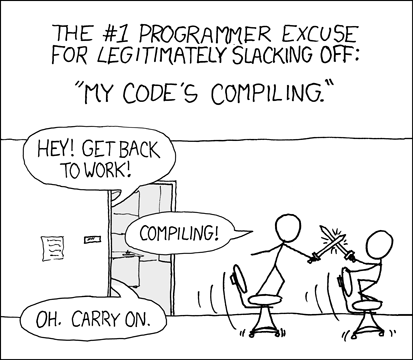
\includegraphics[scale=.7]{img/xkcd/compiling.png}
\caption*{{\small
    \foreignlanguage{english}{
      \textit{\enquote*{Are you stealing those LCDs?} \enquote*{Yeah, but I'm doing it while my code compiles.}\\\hspace*{1mm}\hfill(https://xkcd.com/303)}
    }
  }
}
\end{figure}
